Uno de los primeros pasos para poder realizar cualquier tipo de análisis de datos es necesario graficar los datos, los gráficos permiten ver las distintas propiedades que los datos puedan tener, como lo son patrones, observaciones inusuales (outliers), cambios producidos por el tiempo y las relaciones que se encuentran entre las distintas variables que los datos puedan tener \cite{forecast-time-series-arima}. Por lo que, la selección de un buen grafico para representar los datos resulta ser de gran importancia para poder seleccionar el modelo predictivo más adecuado.

Dentro de esta sección revisaremos los gráficos más relevantes para nuestro estudio:


\begin{itemize}
    \item \textbf{Trama de tiempo (Time plot):} Una de las maneras más practicas y usada para poder entender las series de tiempo es graficar los datos y una de las primeras opciones es una trama de tiempo. Esto quiere decir graficar la datos contra el tiempo de obtención de los datos.
    
    La siguiente figura muestra la cantidad semanal de pasajeros que volaron en la clase económica de Ansett Airlines entre las dos ciudades más grandes de Australia \cite{forecast-time-series-arima}:

    \begin{figure}[H]
        \begin{minipage}[t]{0.9\textwidth}
            \caption{Cantidad semanal de pasajeros que volaron en la clase económica de Ansett Airlines}
            \label{timeplot}        
        \end{minipage}
    
        \vspace{10pt}
    
        \begin{minipage}[b]{0.9\textwidth}
            \centering
            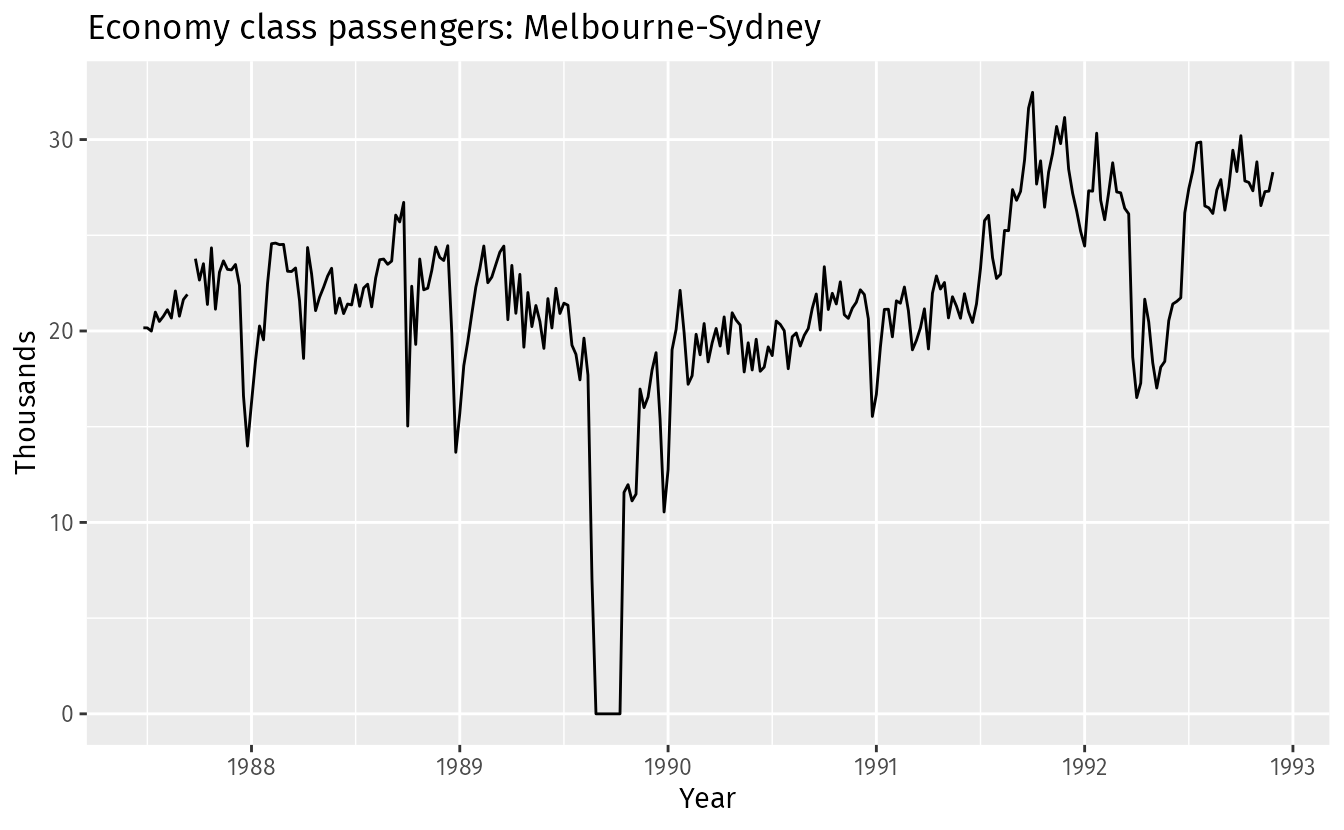
\includegraphics[width=\textwidth]{img/pasajeros-clase-econ-timeplot.png}        
        \end{minipage}
    
        \begin{minipage}[t]{0.9\textwidth}
            Fuente: Forecasting: Principles and Practice (Hyndman y Athanasopoulos, 2023). Recuperado de \url{https://otexts.com/fpp2/time-plots.html}
        \end{minipage}
    \end{figure}
    
    \item \textbf{Patrónes:} Una serie de tiempo puede presentar distintos tipos de patrones a lo largo del tiempo de la observación, y esta puede llegar a presentar este tipo de patrones \cite{forecast-time-series-arima}:
        \begin{itemize}
            \item Tendencia (Trend): Una tendencia existe cuando se presenta un incremento o disminución en los datos dentro de un largo periodo de tiempo, esta tendencia no tiene por qué ser linear, pudiendo tener tendencias positivas o negativas.
            \item Estacional (Seasonal): Un patrón estacional existe cuando la serie de tiempo se ve afectada por factores como el tiempo del año o el día de semana. Gracias a esto se puede identificar que los patrones estacionales tienen una frecuencia conocida que por lo general no varía.
            \item Cíclico (Cyclic): Un patrón cíclico en una serie de tiempo existe cuando los datos presentan incrementos y disminuciones como lo haría un patrón estacional, pero sin una frecuencia conocida o fija, usualmente estos ciclos suelen tener una duración mayor a los de los patrones estacionales. 
        \end{itemize}

        Muchas veces nos encontraremos con series de tiempo que contienen uno o más de estos patrones, por lo que para poder elegir un método predictivo resulta imperativo identificar los patrones presentes en los datos \cite{forecast-time-series-arima}.

    \item \textbf{Tramas de tiempo estacionales (Seasonal plots):} Esta grafica es similar a la trama de tiempo antes mencionada, la diferencia reside en el hecho de que los datos u observaciones están graficadas en contra de cada “estación individual” de tiempo donde se realizó la observación \cite{forecast-time-series-arima}.
    
        En la siguiente figura se representa el valor monetario de las ventas mensuales de medicamentos antidiabéticos en Australia:
        
        \begin{figure}[H]
            \begin{minipage}[t]{0.9\textwidth}
                \caption{Ventas mensuales de medicamentos antidiabéticos en Australia}
                \label{seasonalplot}        
            \end{minipage}
        
            \vspace{10pt}
        
            \begin{minipage}[b]{0.9\textwidth}
                \centering
                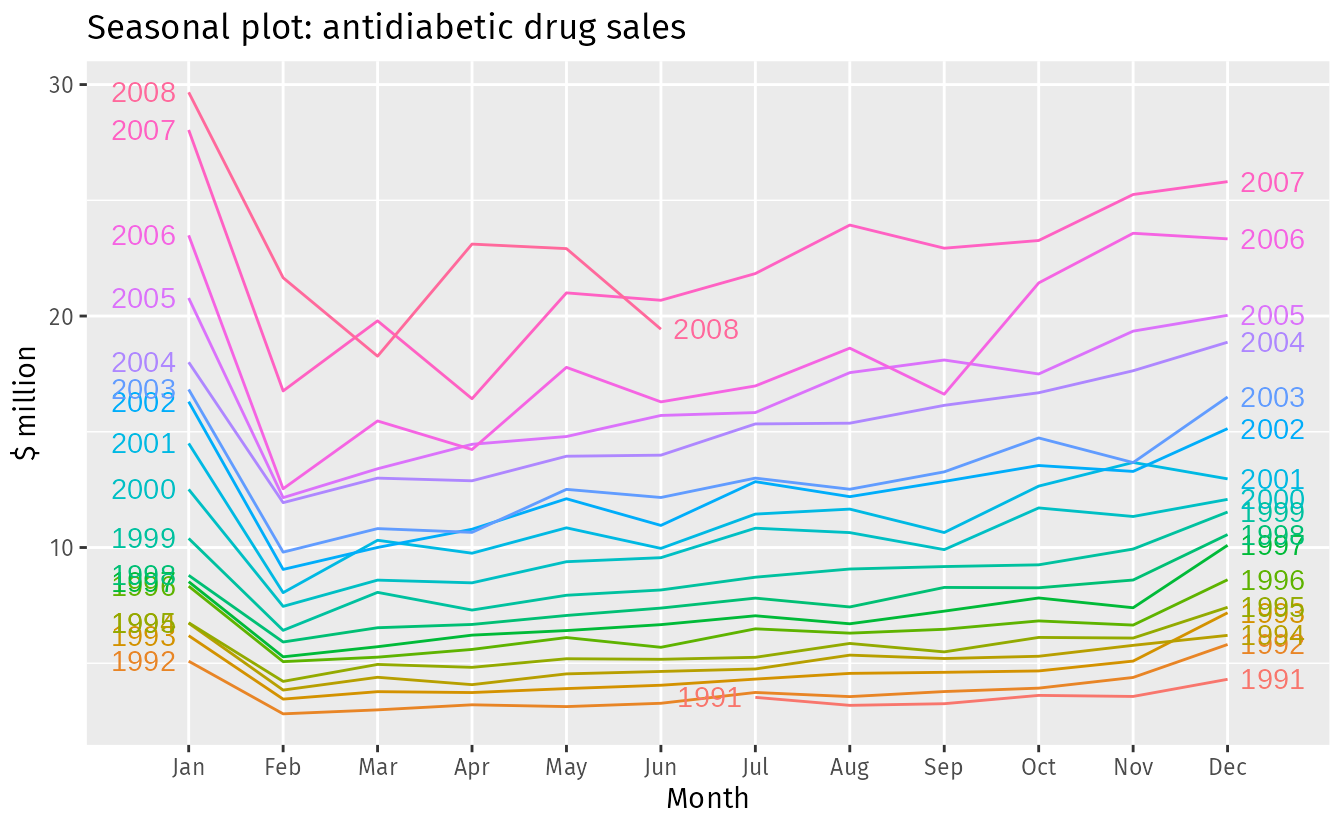
\includegraphics[width=\textwidth]{img/ventas-medicamentos-diab-seasonplot.png}        
            \end{minipage}
        
            \begin{minipage}[t]{0.9\textwidth}
                Fuente: Forecasting: Principles and Practice (Hyndman y Athanasopoulos, 2023). Recuperado de \url{https://otexts.com/fpp2/time-plots.html}
            \end{minipage}
        \end{figure}

        Este tipo de gráficos permite identificar de mejor manera los patrones que no se pudieron apreciar anteriormente en la trama de tiempo, ayuda especialmente para poder observar en que años el patrón de los datos cambia.

    \item \textbf{Gráficos de dispersión (Scatterplots):} Este tipo de grafico permite explorar las relaciones que existen entre series de tiempo, sus distintas variables y como esto afecta a la hora de predecir una serie de tiempo.

        La siguiente figura muestra dos series de tiempo: demanda de electricidad (en GW y temperatura (Celsius)), para 2014 en Victoria, Australia. Las temperaturas son para Melbourne, la ciudad más grande de Victoria, mientras que los valores de demanda son para todo el estado \cite{forecast-time-series-arima}.

        \begin{figure}[H]
            \begin{minipage}[t]{0.9\textwidth}
                \caption{Demanda electrica debido a las temperaturas en 2 ciudades en Australia}
                \label{scatteroplot}        
            \end{minipage}
        
            \vspace{10pt}
        
            \begin{minipage}[b]{0.9\textwidth}
                \centering
                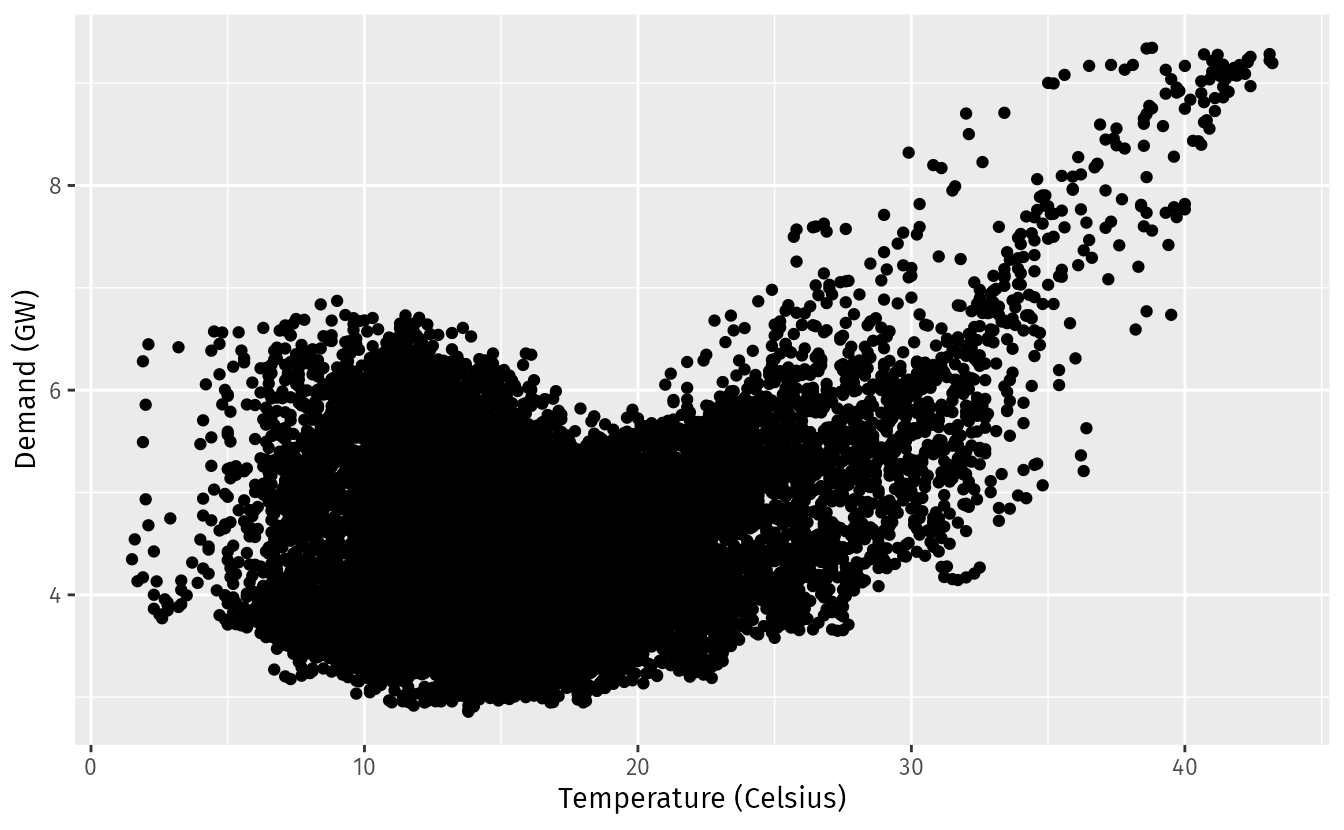
\includegraphics[width=\textwidth]{img/Demanda electrica debido a las temperaturas en 2 ciudades en Australia.png}        
            \end{minipage}
        
            \begin{minipage}[t]{0.9\textwidth}
                Fuente: Forecasting: Principles and Practice (Hyndman y Athanasopoulos, 2023). Recuperado de \url{https://otexts.com/fpp2/time-plots.html}
            \end{minipage}
        \end{figure}

        Este grafico de dispersión es de gran ayuda para visualizar la relación que tienen las variables, y poder entender los datos de mejor manera.

    \item \textbf{Gráficos de desfase (Lag plots):} Este tipo de gráfico representa la observación Y(t) graficada contra la observación Y(t-k) para cada valor de k. Donde en el eje horizontal se muestran valores desfasados de la serie de tiempo \cite{forecast-time-series-arima}. La siguiente figura muestra diagramas de dispersión de la producción trimestral de cerveza australiana:
    
    \begin{figure}[H]
        \begin{minipage}[t]{0.9\textwidth}
            \caption{Producción trimestral de cerveza australiana}
            \label{lagplot}        
        \end{minipage}
    
        \vspace{10pt}
    
        \begin{minipage}[b]{0.9\textwidth}
            \centering
            \includegraphics[width=\textwidth]{img/producción trimestral de cerveza australiana-lagplot.png}        
        \end{minipage}
    
        \begin{minipage}[t]{0.9\textwidth}
            Fuente: Forecasting: Principles and Practice (Hyndman y Athanasopoulos, 2023). Recuperado de \url{https://otexts.com/fpp2/time-plots.html}
        \end{minipage}
    \end{figure}
    
    Los colores representan el cuatrimestre de la variable en el eje vertical. Se puede apreciar que en los desfases 4 y 8 se presenta una fuerte relación de las variables, lo que muestra un patrón estacional fuerte. 

    \item \textbf{Correlación:} El estudio de la correlación explora la relación lineal entre dos variables, resulta de importancia calcularla, esto debido a que entrega que tan intrínsecamente relacionadas se encuentran las variables a analizar \cite{forecast-time-series-arima}. 
    
    A continuación, se presenta la fórmula para conocer el coeficiente de correlación entre dos variables, x e y:

    \begin{equation*}
        r = \frac{\sum{(x_t - \bar{x})(y_t - \bar{y})}}{{\sqrt{\sum{(x_t - \bar{x})}}\sqrt{\sum{(y_t - \bar{y})}}}}
    \end{equation*}    
    
    El valor de r variara entre -1 y 1, dependiendo de que tan fuerte sea la correlación de las variables, mientras más cercano al -1, r representa una correlación negativa, por lo que, si r se encuentra más cercano a 1, esto quiere decir que las variables tienen una correlación positiva \cite{forecast-time-series-arima}.

    \item \textbf{Autocorrelación:} La autocorrelación mide la relación lineal entre valores rezagados de una serie de tiempo. Hay variados coeficientes de autocorrelación, dependiendo de cada panel del Lag plot, por ejemplo, r1 mide la relación entre las variables Y(t) y Y(t-1) y r2 mide la relación entre las variables Y(t) y Y(t-2) y así hasta considerar todos los datos \cite{forecast-time-series-arima}.
    
    Para calcular el valor de r(k), donde T corresponde al largo de la serie de tiempo, se ocupa la siguiente fórmula:

    \begin{equation*}
        r_k = \frac{\sum_{t=k+1}^{T}{(y_t - \bar{y})(y_t-k - \bar{y})}}{\sum_{t=1}^{T}(y_t - \bar{y})^2}
    \end{equation*}  

    De ejemplo, se calcularon los primeros 9 coeficientes de autocorrelación de la producción de cerveza en Australia estudiado en la sección pasada, obteniendo los siguientes valores:

    \begin{figure}[H]
        \begin{minipage}[t]{0.9\textwidth}
            \caption{Coeficientes de autocorrelación de la producción de cerveza en Australia}
            \label{autocorrelaciones1}        
        \end{minipage}
    
        \vspace{10pt}
    
        \begin{minipage}[b]{0.9\textwidth}
            \centering
            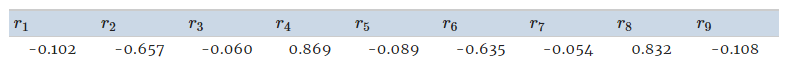
\includegraphics[width=\textwidth]{img/ejemplo_autocorrelaciones.png}        
        \end{minipage}
    
        \begin{minipage}[t]{0.9\textwidth}
            Fuente: Forecasting: Principles and Practice (Hyndman y Athanasopoulos, 2023). Recuperado de \url{https://otexts.com/fpp2/time-plots.html}
        \end{minipage}
    \end{figure}

    Estos coeficientes de autocorrelación son graficados para representar la \textbf{función de autocorrelación (ACF)}, que se muestra a continuación:

    \begin{figure}[H]
        \begin{minipage}[t]{0.9\textwidth}
            \caption{ACF de la produccion trimestral de cerveza}
            \label{autocorrelaciones2}        
        \end{minipage}
    
        \vspace{10pt}
    
        \begin{minipage}[b]{0.9\textwidth}
            \centering
            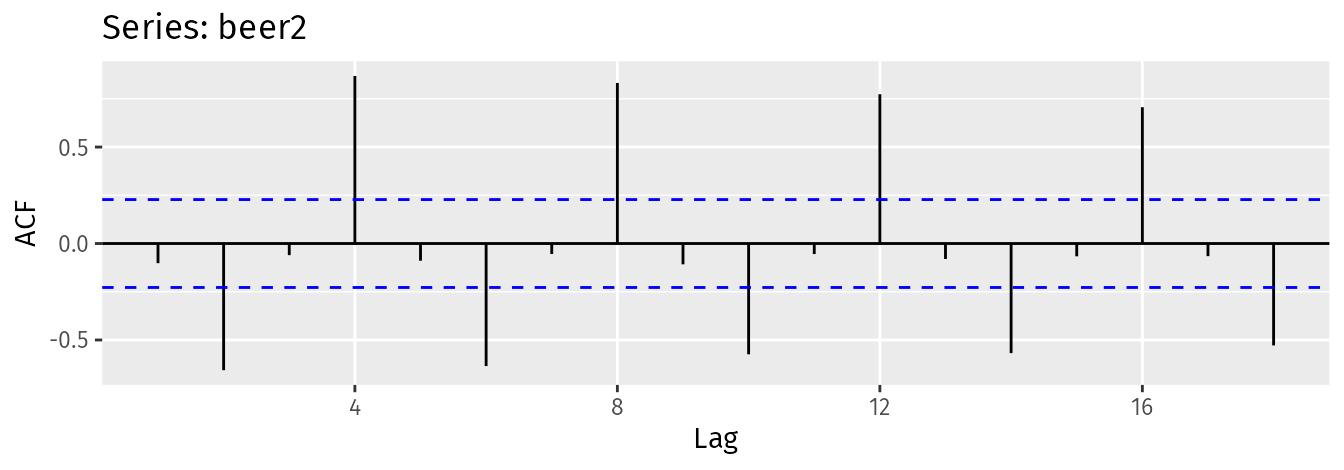
\includegraphics[width=\textwidth]{img/produccion-cerveza-aust-ACF.png}        
        \end{minipage}
    
        \begin{minipage}[t]{0.9\textwidth}
            Fuente: Forecasting: Principles and Practice (Hyndman y Athanasopoulos, 2023). Recuperado de \url{https://otexts.com/fpp2/time-plots.html}
        \end{minipage}
    \end{figure}

    Las líneas azules indican que tan lejos de 0 pueden estar las correlaciones para que estas sean significativas. 
    
    Cuando los datos tienen alguna tendencia, el ACF tiene valores positivos que lentamente van disminuyendo, si los datos presentan un patrón estacional, el ACF mostrara valores más grandes para los desfases estacionales, por lo general siguiendo alguna frecuencia estacional.
    
    Cuando los datos presentan una tendencia y además un patrón estacional, se pueden apreciar ambos efectos \cite{forecast-time-series-arima}. En las siguientes figuras se muestra la demanda mensual de electricidad de Australia, la cual presenta una tendencia y patrón estacional:

    \begin{figure}[H]
        \begin{minipage}[t]{0.9\textwidth}
            \caption{Demanda mensual de electricidad de Australia}
            \label{autocorrelaciones3}        
        \end{minipage}
    
        \vspace{10pt}
    
        \begin{minipage}[b]{0.9\textwidth}
            \centering
            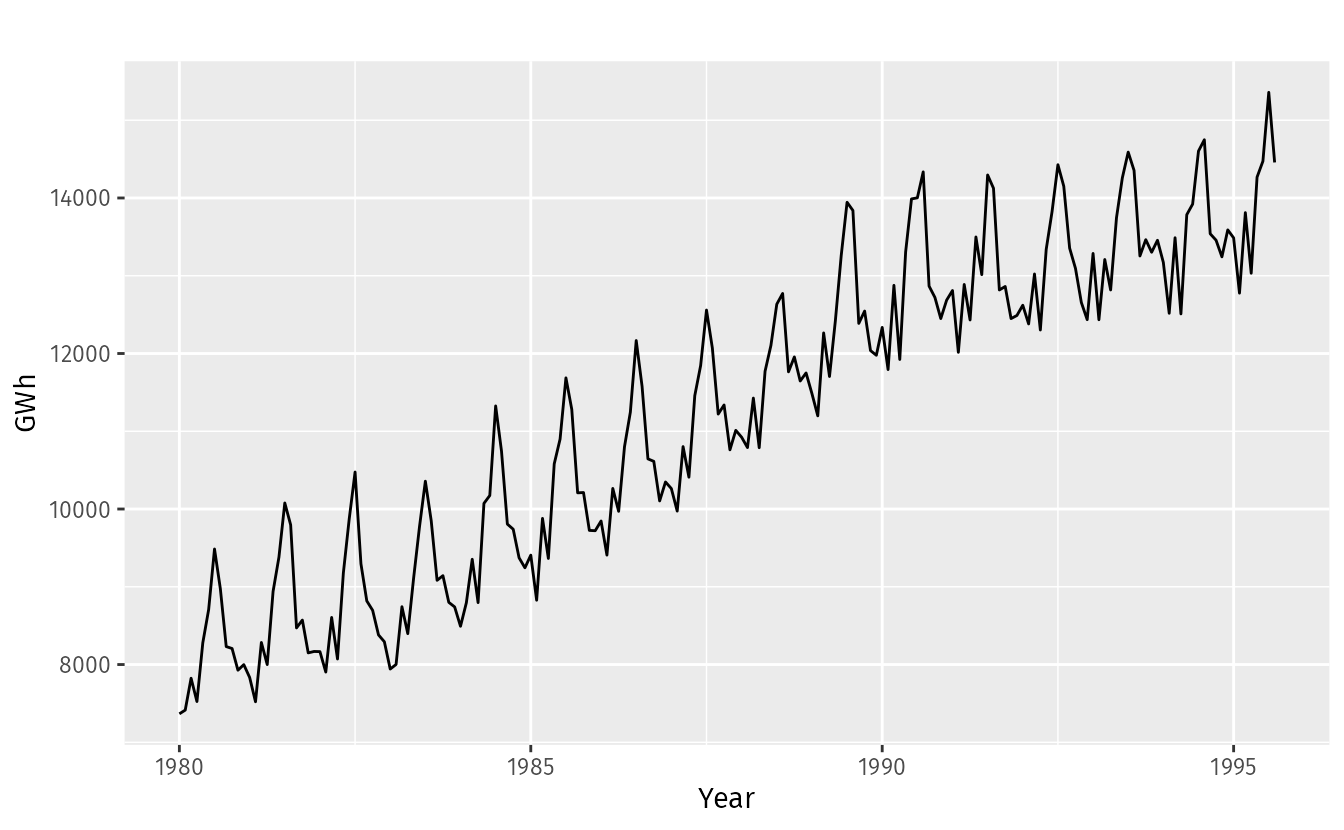
\includegraphics[width=\textwidth]{img/aelec-1-ejemplo.png}        
        \end{minipage}
    
        \begin{minipage}[t]{0.9\textwidth}
            Fuente: Forecasting: Principles and Practice (Hyndman y Athanasopoulos, 2023). Recuperado de \url{https://otexts.com/fpp2/time-plots.html}
        \end{minipage}
    \end{figure}

    \begin{figure}[H]
        \begin{minipage}[t]{0.9\textwidth}
            \caption{ACF demanda mensual de electricidad de Australia}
            \label{autocorrelaciones4}        
        \end{minipage}
    
        \vspace{10pt}
    
        \begin{minipage}[b]{0.9\textwidth}
            \centering
            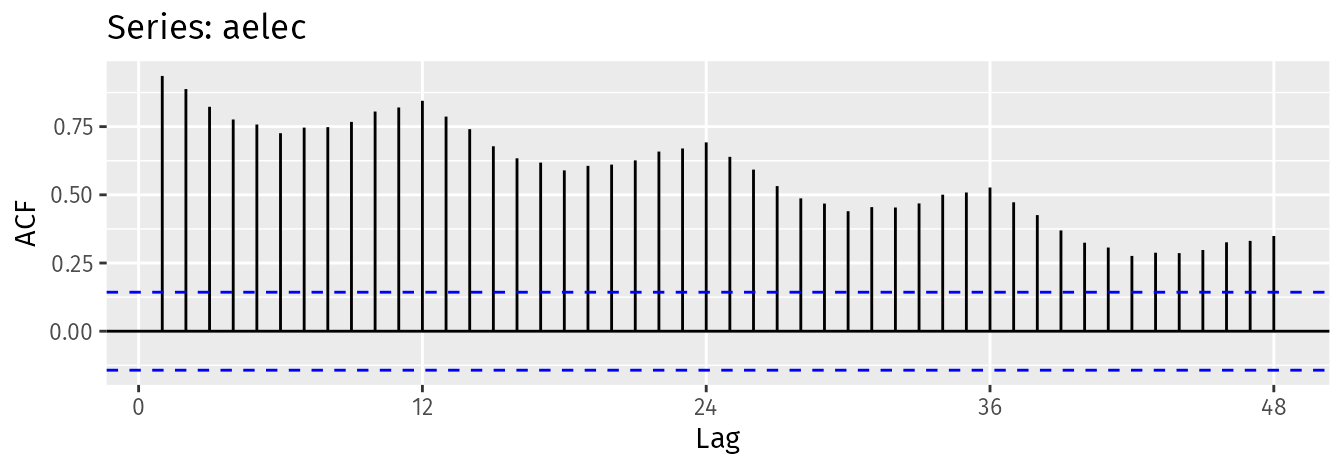
\includegraphics[width=\textwidth]{img/acfelec-1-ejemplo.png}        
        \end{minipage}
    
        \begin{minipage}[t]{0.9\textwidth}
            Fuente: Forecasting: Principles and Practice (Hyndman y Athanasopoulos, 2023). Recuperado de \url{https://otexts.com/fpp2/time-plots.html}
        \end{minipage}
    \end{figure}

    En el ACF se puede apreciar una tendencia, esto debido a que los valores van disminuyendo lentamente, mientras que la forma de ondas es debido a la estacionalidad que se presenta cada año.

    \item \textbf{Ruido Blanco (White Noise):} Las series de tiempo que no tienen autocorrelación son llamadas ruido blanco, para esto se espera que cada autocorrelación sea lo más cercana a 0. Debido a la variación que estos valores pueden tener, por lo que para que una serie de tiempo sea considerada ruido blanco, se espera que el 95\% de sus valores representados en el ACF estén unos limites demarcados por $\pm{2}/\sqrt{T}$, donde T corresponde al largo de la serie de tiempo, estos limites se encuentran representados comúnmente por líneas azules en el ACF. Por consiguiente, si un valor o más se encuentra fuera de los limites o el más del 5\% de los valores estén fuera de los límites, la serie de tiempo en cuestión probablemente no sea ruido blanco.

    \begin{figure}[H]
        \begin{minipage}[t]{0.9\textwidth}
            \caption{Ruido blanco}
            \label{whitenoise1}        
        \end{minipage}
    
        \vspace{10pt}
    
        \begin{minipage}[b]{0.9\textwidth}
            \centering
            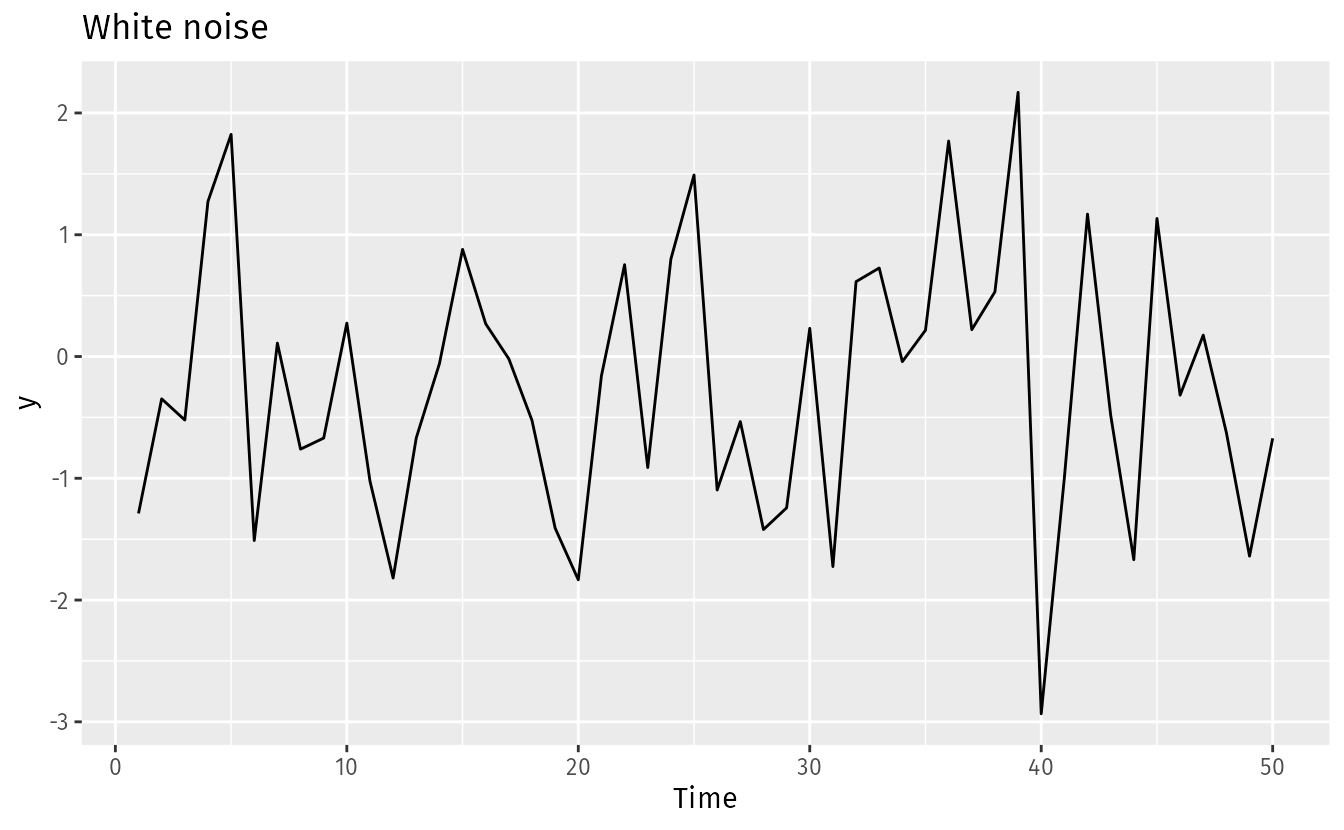
\includegraphics[width=\textwidth]{img/wnoise-1.png}        
        \end{minipage}
    
        \begin{minipage}[t]{0.9\textwidth}
            Fuente: Forecasting: Principles and Practice (Hyndman y Athanasopoulos, 2023). Recuperado de \url{https://otexts.com/fpp2/time-plots.html}
        \end{minipage}
    \end{figure}

    \begin{figure}[H]
        \begin{minipage}[t]{0.9\textwidth}
            \caption{ACF Ruido blanco}
            \label{whitenoise2}        
        \end{minipage}
    
        \vspace{10pt}
    
        \begin{minipage}[b]{0.9\textwidth}
            \centering
            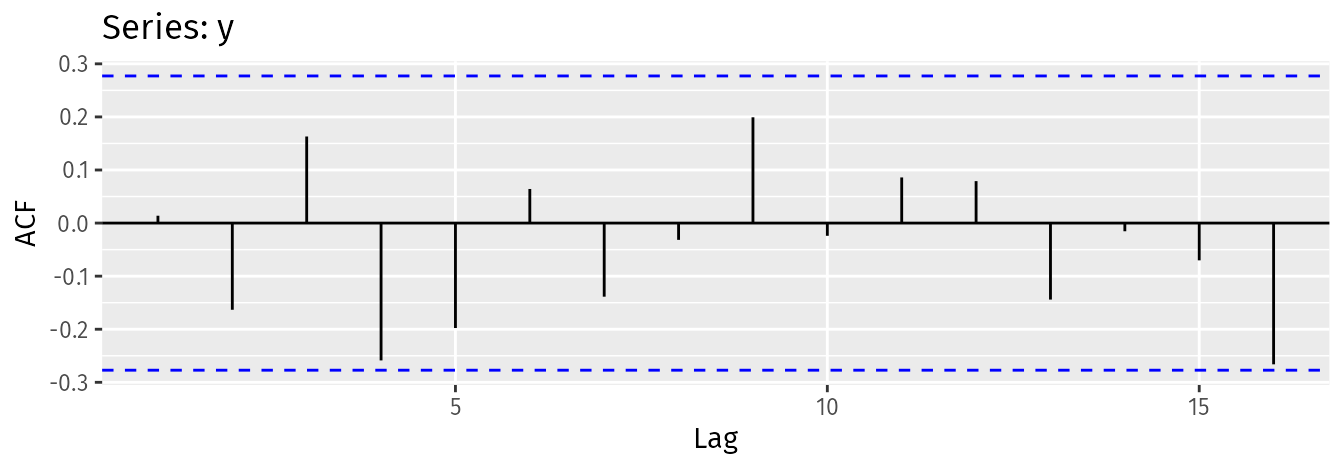
\includegraphics[width=\textwidth]{img/wnoiseacf-1.png}        
        \end{minipage}
    
        \begin{minipage}[t]{0.9\textwidth}
            Fuente: Forecasting: Principles and Practice (Hyndman y Athanasopoulos, 2023). Recuperado de \url{https://otexts.com/fpp2/time-plots.html}
        \end{minipage}
    \end{figure}

    Teniendo en cuenta que T = 50, por lo tanto, los limites están calculados como $\pm{2}/\sqrt{50}  = \pm{0.28}$. En el ACF se puede apreciar que todos los coeficientes de autocorrelación se encuentran dentro estos límites, concluyendo que los datos son ruido blanco.

\end{itemize}

